% Options for packages loaded elsewhere
\PassOptionsToPackage{unicode}{hyperref}
\PassOptionsToPackage{hyphens}{url}
%
\documentclass[
]{article}
\usepackage{amsmath,amssymb}
\usepackage{lmodern}
\usepackage{ifxetex,ifluatex}
\ifnum 0\ifxetex 1\fi\ifluatex 1\fi=0 % if pdftex
  \usepackage[T1]{fontenc}
  \usepackage[utf8]{inputenc}
  \usepackage{textcomp} % provide euro and other symbols
\else % if luatex or xetex
  \usepackage{unicode-math}
  \defaultfontfeatures{Scale=MatchLowercase}
  \defaultfontfeatures[\rmfamily]{Ligatures=TeX,Scale=1}
\fi
% Use upquote if available, for straight quotes in verbatim environments
\IfFileExists{upquote.sty}{\usepackage{upquote}}{}
\IfFileExists{microtype.sty}{% use microtype if available
  \usepackage[]{microtype}
  \UseMicrotypeSet[protrusion]{basicmath} % disable protrusion for tt fonts
}{}
\makeatletter
\@ifundefined{KOMAClassName}{% if non-KOMA class
  \IfFileExists{parskip.sty}{%
    \usepackage{parskip}
  }{% else
    \setlength{\parindent}{0pt}
    \setlength{\parskip}{6pt plus 2pt minus 1pt}}
}{% if KOMA class
  \KOMAoptions{parskip=half}}
\makeatother
\usepackage{xcolor}
\IfFileExists{xurl.sty}{\usepackage{xurl}}{} % add URL line breaks if available
\IfFileExists{bookmark.sty}{\usepackage{bookmark}}{\usepackage{hyperref}}
\hypersetup{
  pdftitle={UAE Manuscript 1 - Medical and Behavioral},
  hidelinks,
  pdfcreator={LaTeX via pandoc}}
\urlstyle{same} % disable monospaced font for URLs
\usepackage[margin=1in]{geometry}
\usepackage{graphicx}
\makeatletter
\def\maxwidth{\ifdim\Gin@nat@width>\linewidth\linewidth\else\Gin@nat@width\fi}
\def\maxheight{\ifdim\Gin@nat@height>\textheight\textheight\else\Gin@nat@height\fi}
\makeatother
% Scale images if necessary, so that they will not overflow the page
% margins by default, and it is still possible to overwrite the defaults
% using explicit options in \includegraphics[width, height, ...]{}
\setkeys{Gin}{width=\maxwidth,height=\maxheight,keepaspectratio}
% Set default figure placement to htbp
\makeatletter
\def\fps@figure{htbp}
\makeatother
\setlength{\emergencystretch}{3em} % prevent overfull lines
\providecommand{\tightlist}{%
  \setlength{\itemsep}{0pt}\setlength{\parskip}{0pt}}
\setcounter{secnumdepth}{5}
\usepackage{fullpage}
\usepackage{graphicx}
\usepackage{subcaption}
\usepackage{float}
\usepackage{placeins}
\usepackage{caption}
\usepackage{mathtools}
\usepackage{multirow}
\usepackage{amssymb}
\usepackage{amsmath}
\usepackage{bigstrut}
\usepackage{geometry}
\usepackage{pdflscape}
\setlength{skip}{1em}
\usepackage{booktabs}
\usepackage{longtable}
\usepackage{array}
\usepackage{multirow}
\usepackage{wrapfig}
\usepackage{float}
\usepackage{colortbl}
\usepackage{pdflscape}
\usepackage{tabu}
\usepackage{threeparttable}
\usepackage{threeparttablex}
\usepackage[normalem]{ulem}
\usepackage{makecell}
\usepackage{xcolor}
\ifluatex
  \usepackage{selnolig}  % disable illegal ligatures
\fi

\title{UAE Manuscript 1 - Medical and Behavioral}
\author{}
\date{\vspace{-2.5em}}

\begin{document}
\maketitle

{
\setcounter{tocdepth}{2}
\tableofcontents
}
\textbackslash begin\{document\}

\clearpage

\hypertarget{measurement-of-weight-status}{%
\section{Measurement of Weight
Status}\label{measurement-of-weight-status}}

We decided to use the International Obesity Task Force (IOTF)
designation of weight status for the sample. They use smoothed,
sex-specific BMI curves meant to match the the BMI cutoffs for
overweight (OW; 25 \(kg/m^2\)) and obesity (OB; 30 \(kg/m^2\)) at age 18
yrs.

Rather than BMI-zscore or BMI-percentile, we chose to use percent of
overweight cutoff because recent studies shows it has a tighter
association with measured adiposity:

BMI \(\%\) of overweight =
\(\frac{child BMI}{BMI\: at\: age-\: and\: sex-\: adjusted\: overweight\: cutoff}*100\)

\textless100 \(\%\) - indicates child BMI is below the overweight cutoff
for age and sex (i.e., has healthy weight) 100 \(\%\) - indicates child
BMI is the same as the overweight cutoff for age and sex \textgreater100
\(\%\) - indicates child BMI is above the overweight cutoff for age and
sex (i.e., has overweight or obesity)

\FloatBarrier

Density plot of percent of overweight by sex. The shaded regions
indicated those with healthy weight (blue), overweight (yellow), and
obesity (red). The points show denisity of participants by sex (purple
circles = female, orange triangles = males).

\FloatBarrier

\hypertarget{participant-characteristics}{%
\section{Participant
Characteristics}\label{participant-characteristics}}

\begin{table}[!h]

\caption{\label{tab:Demo_OB_tab}Demographic Characteristics by Weight Status}
\centering
\begin{tabular}[t]{lllllll}
\toprule
Characteristic & N & HW & OW & OB & ANOVA & chi/fisher\\
\midrule
Age\_yr & 107 & 11.85 [8.02 - 17.37] & 12.84 [8.15 - 17.54] & 13.69 [7.31 - 17.84] & 0.010 & \\
BMI & 107 & 17.15 [12.71 - 22.72] & 24.03 [18.70 - 28.86] & 35.08 [21.87 - 55.52] & 0.000 & \\
IOTF\_pOWcutoff & 107 & 80.86 [63.95 - 98.26] & 109.66 [100.39 - 120.73] & 155.80 [122.38 - 239.00] & 0.000 & \\
hw\_ratio & 83 & 1.18 [0.77 - 1.34] & 1.14 [1.00 - 1.30] & 1.23 [1.01 - 3.52] & 0.515 & \\
\hspace{1em}Unknown &  & 14 & 7 & 3 &  & \\
\addlinespace
Father\_ed & 102 & 12.79 [6.00 - 18.00] & 13.60 [6.00 - 18.00] & 12.20 [0.00 - 18.00] & 0.285 & \\
\hspace{1em}Unknown &  & 3 & 0 & 2 &  & \\
Mother\_ed & 99 & 13.38 [3.00 - 18.00] & 13.93 [9.00 - 18.00] & 12.40 [0.00 - 18.00] & 0.184 & \\
\hspace{1em}Unknown &  & 4 & 2 & 2 &  & \\
Month\_AED & 99 &  &  &  &  & 0.844\\
\addlinespace
\hspace{1em}<25,000 AED &  & 10 (27\%) & 10 (34\%) & 11 (33\%) &  & \\
\hspace{1em}25,000 - 55,000 AED &  & 21 (57\%) & 13 (45\%) & 19 (58\%) &  & \\
\hspace{1em}55,000 - 75,000 AED &  & 2 (5.4\%) & 3 (10\%) & 1 (3.0\%) &  & \\
\hspace{1em}> 75,000 AED &  & 4 (11\%) & 3 (10\%) & 2 (6.1\%) &  & \\
\hspace{1em}Unknown &  & 4 & 0 & 4 &  & \\
\addlinespace
DadNationality & 101 &  &  &  &  & 0.095\\
\hspace{1em}Emirati &  & 40 (100\%) & 25 (96\%) & 33 (94\%) &  & \\
\hspace{1em}Omani &  & 0 (0\%) & 1 (3.8\%) & 0 (0\%) &  & \\
\hspace{1em}Yemeni &  & 0 (0\%) & 0 (0\%) & 2 (5.7\%) &  & \\
\hspace{1em}Unknown &  & 1 & 3 & 2 &  & \\
\addlinespace
MomNationality & 104 &  &  &  &  & 0.649\\
\hspace{1em}Emirati &  & 38 (93\%) & 26 (93\%) & 32 (91\%) &  & \\
\hspace{1em}Omani &  & 0 (0\%) & 1 (3.6\%) & 0 (0\%) &  & \\
\hspace{1em}Yemeni &  & 0 (0\%) & 0 (0\%) & 1 (2.9\%) &  & \\
\hspace{1em}Moroccan &  & 1 (2.4\%) & 0 (0\%) & 1 (2.9\%) &  & \\
\addlinespace
\hspace{1em}Egyptian &  & 2 (4.9\%) & 0 (0\%) & 1 (2.9\%) &  & \\
\hspace{1em}Bahrani &  & 0 (0\%) & 1 (3.6\%) & 0 (0\%) &  & \\
\hspace{1em}Unknown &  & 0 & 1 & 2 &  & \\
\bottomrule
\multicolumn{7}{l}{\rule{0pt}{1em}\textsuperscript{1} Mean [Range]; n (\%)}\\
\end{tabular}
\end{table}
\FloatBarrier

\hypertarget{associations-between-demographics-and-percent-of-overweight-cutoff}{%
\subsection{Associations between Demographics and Percent of Overweight
Cutoff}\label{associations-between-demographics-and-percent-of-overweight-cutoff}}

\begin{table}[!h]

\caption{\label{tab:IOTF_pOWcutoff_demo_cors}Correlations between percent of overweight cuttoff and demographic characteristics}
\centering
\begin{tabular}[t]{lllll}
\toprule
  & Age\_yr & Father\_ed & Mother\_ed & IOTF\_pOWcutoff\\
\midrule
Age\_yr &  &  &  & \\
Father\_ed & -0.02 &  &  & \\
Mother\_ed & -0.2* & 0.51* &  & \\
IOTF\_pOWcutoff & 0.26* & -0.07 & -0.15 & \\
\bottomrule
\end{tabular}
\end{table}

\FloatBarrier

Only child age was associated with percent of overweight cutoff - older
children tended to have higher percent of overweight cutoff indicating
older children were more likely to have overweight or obesity. There was
no association with father or mother education level, which differs from
finding in the US. Hip to waist ratio was also not associated with
percent of overweight cutoff.

\FloatBarrier

\begin{verbatim}
Anova Table (Type III tests)

Response: IOTF_pOWcutoff
            Sum Sq Df  F value Pr(>F)    
(Intercept) 406511  1 282.6340 <2e-16 ***
Month_AED     1046  3   0.2424 0.8665    
Residuals   136638 95                    
---
Signif. codes:  0 '***' 0.001 '**' 0.01 '*' 0.05 '.' 0.1 ' ' 1
\end{verbatim}

\FloatBarrier

There was no difference in percent of overweight by monthly income
category.

\FloatBarrier

\clearpage

\hypertarget{medical-comorbidities}{%
\section{Medical Comorbidities}\label{medical-comorbidities}}

\begin{table}[!h]

\caption{\label{tab:Med_OB_tab}Medical Comorbidites by Weight Status}
\centering
\begin{tabular}[t]{lllll}
\toprule
Characteristic & N & HW, N = 41 & OW, N = 29 & OB, N = 37\\
\midrule
nComorbid & 107 & 2.05 [0.00 - 4.00] & 2.24 [1.00 - 4.00] & 2.19 [0.00 - 4.00]\\
VitDdeficiency & 107 &  &  & \\
\hspace{1em}Y &  & 36 (88\%) & 29 (100\%) & 33 (89\%)\\
\hspace{1em}N &  & 5 (12\%) & 0 (0\%) & 4 (11\%)\\
Anemia & 40 &  &  & \\
\addlinespace
\hspace{1em}Iron Deficiency Anemia (ID) &  & 9 (39\%) & 7 (70\%) & 5 (71\%)\\
\hspace{1em}Thalassemia Minor (TM) &  & 2 (8.7\%) & 1 (10\%) & 0 (0\%)\\
\hspace{1em}G6PD Deficiency &  & 1 (4.3\%) & 0 (0\%) & 0 (0\%)\\
\hspace{1em}ID + TM &  & 1 (4.3\%) & 1 (10\%) & 0 (0\%)\\
\hspace{1em}ID + G6PD Deficiency &  & 1 (4.3\%) & 0 (0\%) & 0 (0\%)\\
\addlinespace
\hspace{1em}Unspecified Anemia &  & 9 (39\%) & 1 (10\%) & 2 (29\%)\\
\hspace{1em}Unknown &  & 18 & 19 & 30\\
Hyperlipidemia & 12 &  &  & \\
\hspace{1em}Hyperlipidemia &  & 0 (NA\%) & 5 (100\%) & 6 (86\%)\\
\hspace{1em}Hyperlipidemia - Mixed &  & 0 (NA\%) & 0 (0\%) & 1 (14\%)\\
\addlinespace
\hspace{1em}Unknown &  & 41 & 24 & 30\\
ThyroidConditions & 25 &  &  & \\
\hspace{1em}Abnormal Function &  & 5 (71\%) & 4 (44\%) & 5 (56\%)\\
\hspace{1em}Autoimmune Thyroiditis &  & 1 (14\%) & 2 (22\%) & 2 (22\%)\\
\hspace{1em}Autoimmune Hypothyroidism &  & 0 (0\%) & 0 (0\%) & 0 (0\%)\\
\addlinespace
\hspace{1em}Unspecified Hypothyroidism &  & 1 (14\%) & 2 (22\%) & 2 (22\%)\\
\hspace{1em}Goiter &  & 0 (0\%) & 1 (11\%) & 0 (0\%)\\
\hspace{1em}Unknown &  & 34 & 20 & 28\\
GlycemicStatus & 28 &  &  & \\
\hspace{1em}Impaired Fasting Glucose &  & 4 (57\%) & 8 (73\%) & 7 (70\%)\\
\addlinespace
\hspace{1em}Impaired Glucose Tolerance Test &  & 2 (29\%) & 2 (18\%) & 3 (30\%)\\
\hspace{1em}Type-1 Diabetes &  & 1 (14\%) & 1 (9.1\%) & 0 (0\%)\\
\hspace{1em}Unknown &  & 34 & 18 & 27\\
Acanthosis Nigricans & 8 & 1 (100\%) & 0 (NA\%) & 7 (100\%)\\
\hspace{1em}Unknown &  & 40 & 29 & 30\\
\addlinespace
Hypertension & 3 &  &  & \\
\hspace{1em}Essential Primary Hypertension &  & 0 (NA\%) & 0 (NA\%) & 2 (67\%)\\
\hspace{1em}High Blood Pressure &  & 0 (NA\%) & 0 (NA\%) & 1 (33\%)\\
\hspace{1em}Unknown &  & 41 & 29 & 34\\
Metabolic Syndrome & 2 & 1 (100\%) & 0 (NA\%) & 1 (100\%)\\
\addlinespace
\hspace{1em}Unknown &  & 40 & 29 & 36\\
Growth.Stature & 10 &  &  & \\
\hspace{1em}Failure To Thrive (FT) &  & 1 (14\%) & 0 (0\%) & 0 (0\%)\\
\hspace{1em}Growth Hormone Deficency &  & 1 (14\%) & 0 (0\%) & 0 (0\%)\\
\hspace{1em}Short Stature &  & 3 (43\%) & 1 (100\%) & 2 (100\%)\\
\addlinespace
\hspace{1em}FT + ShortStature + Underweight &  & 1 (14\%) & 0 (0\%) & 0 (0\%)\\
\hspace{1em}Short Stature + Precocious Puberty &  & 1 (14\%) & 0 (0\%) & 0 (0\%)\\
\hspace{1em}Unknown &  & 34 & 28 & 35\\
PCOS & 4 &  &  & \\
\hspace{1em}PCOS &  & 1 (50\%) & 0 (NA\%) & 1 (50\%)\\
\addlinespace
\hspace{1em}Hirsutism &  & 0 (0\%) & 0 (NA\%) & 1 (50\%)\\
\hspace{1em}Hirsutism + Unspecified Ovarian Cysts &  & 1 (50\%) & 0 (NA\%) & 0 (0\%)\\
\hspace{1em}Unknown &  & 39 & 29 & 35\\
\bottomrule
\multicolumn{5}{l}{\rule{0pt}{1em}\textsuperscript{1} Mean [Range]; n (\%)}\\
\end{tabular}
\end{table}

\FloatBarrier

\hypertarget{association-betwen-number-of-comorbidities-and-percent-of-overweight-cutoff}{%
\subsection{Association betwen Number of Comorbidities and Percent of
Overweight
Cutoff}\label{association-betwen-number-of-comorbidities-and-percent-of-overweight-cutoff}}

\begin{verbatim}
    Pearson's product-moment correlation

data:  UAE_allDat$IOTF_pOWcutoff and UAE_allDat$nComorbid
t = 0.74423, df = 105, p-value = 0.4584
alternative hypothesis: true correlation is not equal to 0
95 percent confidence interval:
 -0.1190571  0.2587387
sample estimates:
       cor 
0.07243876 
\end{verbatim}

\FloatBarrier

There was no association between percent of overweight cutoff and number
of comorbidities

\FloatBarrier

\hypertarget{differences-in-percent-of-overweight-cutoff-by-presenceabsence-of-anemia-thyroid-dysfunction-and-impaired-glucose-function}{%
\subsubsection{Differences in Percent of Overweight Cutoff by
Presence/Absence of: Anemia, Thyroid Dysfunction, and Impaired Glucose
Function}\label{differences-in-percent-of-overweight-cutoff-by-presenceabsence-of-anemia-thyroid-dysfunction-and-impaired-glucose-function}}

\begin{table}[!h]

\caption{\label{tab:IOTF_pOWcutoff_MedComorbid_ttests}t-tests for percent of overweight by absence vs presence of medical comorbidity}
\centering
\begin{tabular}[t]{lrrrrrl}
\toprule
  & AbsentMean & PresentMean & t & df & pvalue & sig\\
\midrule
VitD Deficiency & 114.56 & 114.84 & -0.02 & 9.25 & 0.984 & \\
Anemia & 122.62 & 101.12 & 3.01 & 81.89 & 0.004 & **\\
Thyroid Dysfunction & 113.40 & 118.44 & -0.59 & 39.42 & 0.559 & \\
Glycemic Status & 112.51 & 120.43 & -0.86 & 39.25 & 0.393 & \\
\bottomrule
\end{tabular}
\end{table}
\FloatBarrier

There were no difference in percent of overweight cutoff by
presence/absence of Thyroid dysfunction or impaired glucose function.
However, those with anemia tended to have lower percent of overweight.
The mean with anemia was 101\% indicating children were overweight on
average. The mean for those without anemia were 123\%, indicating the
children were above the overweight cutoff.

\FloatBarrier
\clearpage

\hypertarget{family-history}{%
\section{Family History}\label{family-history}}

\begin{table}[!h]

\caption{\label{tab:Fam_OB_tab}Family History by Weight Status}
\centering
\begin{tabular}[t]{lllll}
\toprule
Characteristic & N & HW, N = 41 & OW, N = 29 & OB, N = 37\\
\midrule
Fam\_OB\_YN & 101 &  &  & \\
\hspace{1em}yes &  & 18 (49\%) & 21 (72\%) & 31 (89\%)\\
\hspace{1em}no &  & 19 (51\%) & 8 (28\%) & 4 (11\%)\\
\hspace{1em}Unknown &  & 4 & 0 & 2\\
nFam\_Obesity & 107 & 1.15 [0.00 - 6.00] & 1.59 [0.00 - 4.00] & 2.70 [0.00 - 7.00]\\
\addlinespace
Mother & 107 & 5 (12\%) & 2 (6.9\%) & 11 (30\%)\\
Father & 107 & 6 (15\%) & 4 (14\%) & 11 (30\%)\\
Grandmother & 107 & 11 (27\%) & 9 (31\%) & 13 (35\%)\\
Grandfather & 107 & 0 (0\%) & 2 (6.9\%) & 4 (11\%)\\
Sister & 107 & 5 (12\%) & 3 (10\%) & 8 (22\%)\\
\addlinespace
Brother & 107 & 5 (12\%) & 3 (10\%) & 17 (46\%)\\
Aunt & 107 & 10 (24\%) & 17 (59\%) & 18 (49\%)\\
Uncle & 107 & 5 (12\%) & 6 (21\%) & 18 (49\%)\\
Fam\_ED\_YN & 96 &  &  & \\
\hspace{1em}yes &  & 2 (5.6\%) & 5 (19\%) & 4 (12\%)\\
\addlinespace
\hspace{1em}no &  & 34 (94\%) & 22 (81\%) & 29 (88\%)\\
\hspace{1em}Unknown &  & 5 & 2 & 4\\
nFam\_EatingDisorder & 107 & 0.05 [0.00 - 1.00] & 0.28 [0.00 - 2.00] & 0.35 [0.00 - 7.00]\\
Mother & 107 & 0 (0\%) & 0 (0\%) & 1 (2.7\%)\\
Father & 107 & 0 (0\%) & 0 (0\%) & 2 (5.4\%)\\
\addlinespace
Grandmother & 107 & 1 (2.4\%) & 1 (3.4\%) & 2 (5.4\%)\\
Grandfather & 107 & 0 (0\%) & 1 (3.4\%) & 1 (2.7\%)\\
Sister & 107 & 1 (2.4\%) & 1 (3.4\%) & 0 (0\%)\\
Brother & 107 & 0 (0\%) & 1 (3.4\%) & 1 (2.7\%)\\
Aunt & 107 & 0 (0\%) & 3 (10\%) & 4 (11\%)\\
\addlinespace
Uncle & 107 & 0 (0\%) & 1 (3.4\%) & 2 (5.4\%)\\
\bottomrule
\multicolumn{5}{l}{\rule{0pt}{1em}\textsuperscript{1} n (\%); Mean [Range]}\\
\end{tabular}
\end{table}

\FloatBarrier

\hypertarget{association-betwen-family-history-and-percent-of-overweight-cutoff}{%
\subsection{Association Betwen Family History and Percent of Overweight
Cutoff}\label{association-betwen-family-history-and-percent-of-overweight-cutoff}}

\begin{table}[!h]

\caption{\label{tab:IOTF_pOWcutoff_FamHistory_ttests}t-tests for percent of overweight by absence vs presence of family history}
\centering
\begin{tabular}[t]{lrrrrrl}
\toprule
  & No & Yes & t & df & pvalue & sig\\
\midrule
Family History of Obesity & 125.09 & 94.77 & 4.83 & 87.92 & 0.000 & ***\\
Family History of Eating Disorder & 116.69 & 114.82 & 0.18 & 14.13 & 0.856 & \\
\bottomrule
\end{tabular}
\end{table}

\FloatBarrier

There was no differences in percent of overweight for those whose
families had a history of eating disorder (reported by parent). There
was a significant difference in percent of overweight between families
that reported a history of obesity (`Yes') and those who did not (`No').
Those without a family history of obesity had a mean percent of
overweight equal to 94\%, indicating the children had healthy weight on
average. Children with a family history of obesity had a mean percent of
overweight equal to 124\%, indicating the children had overweight or
obesity.

\FloatBarrier

\begin{table}[!h]

\caption{\label{tab:IOTF_pOWcutoff_nFam_cor}Correlations between number of family members with history and percent of overweight}
\centering
\begin{tabular}[t]{llll}
\toprule
  & nFam\_Obesity & nFam\_EatingDisorder & IOTF\_pOWcutoff\\
\midrule
nFam\_Obesity &  &  & \\
nFam\_EatingDisorder & 0.37* &  & \\
IOTF\_pOWcutoff & 0.43* & 0.09 & \\
\bottomrule
\end{tabular}
\end{table}

\FloatBarrier

Percent of overweight cutoff was not associated with reported number of
family members with an perceived to have had an eating disorder but was
associated with family history of obesity.

\FloatBarrier

\hypertarget{sensitivity-tests}{%
\subsubsection{Sensitivity Tests}\label{sensitivity-tests}}

\begin{table}[!h]

\caption{\label{tab:IOTF_pOWcutoff_nFam_poisson}Linear Model: Peer Problems (raw) - SES category + Maternal Education + Age + Sex + pOWcutoff}
\centering
\begin{tabular}[t]{lrrrrrrrl}
\toprule
  & b & e\textasciicircum{}b & se & e\textasciicircum{}2.5 CI & e\textasciicircum{}97.5 CI & z & p &  \\
\midrule
(Intercept) & -0.180 & 0.835 & 0.577 & 0.266 & 2.558 & -0.313 & 0.754 & \\
Month\_AED25,000 - 55,000 AED & 0.113 & 1.120 & 0.182 & 0.788 & 1.610 & 0.622 & 0.534 & \\
Month\_AED55,000 - 75,000 AED & 0.380 & 1.462 & 0.307 & 0.779 & 2.611 & 1.239 & 0.215 & \\
Month\_AED> 75,000 AED & -0.127 & 0.880 & 0.372 & 0.404 & 1.761 & -0.342 & 0.732 & \\
Mother\_ed & -0.029 & 0.971 & 0.024 & 0.928 & 1.019 & -1.221 & 0.222 & .\\
\addlinespace
Age\_yr & 0.011 & 1.011 & 0.031 & 0.950 & 1.075 & 0.335 & 0.738 & \\
sexM & -0.111 & 0.895 & 0.159 & 0.654 & 1.218 & -0.703 & 0.482 & \\
IOTF\_pOWcutoff & 0.008 & 1.008 & 0.002 & 1.005 & 1.012 & 4.360 & 0.000 & ***\\
\bottomrule
\end{tabular}
\end{table}

\FloatBarrier

After controlling for family income, mother education, child age, and
child sex, percent of overweight showed a trend-level association with
number of family members with history of obesity. A child with 110\% of
overweight, compared to 100\%, would have 1.08 times the odds of having
an additional family member with a history of obesity.

\FloatBarrier

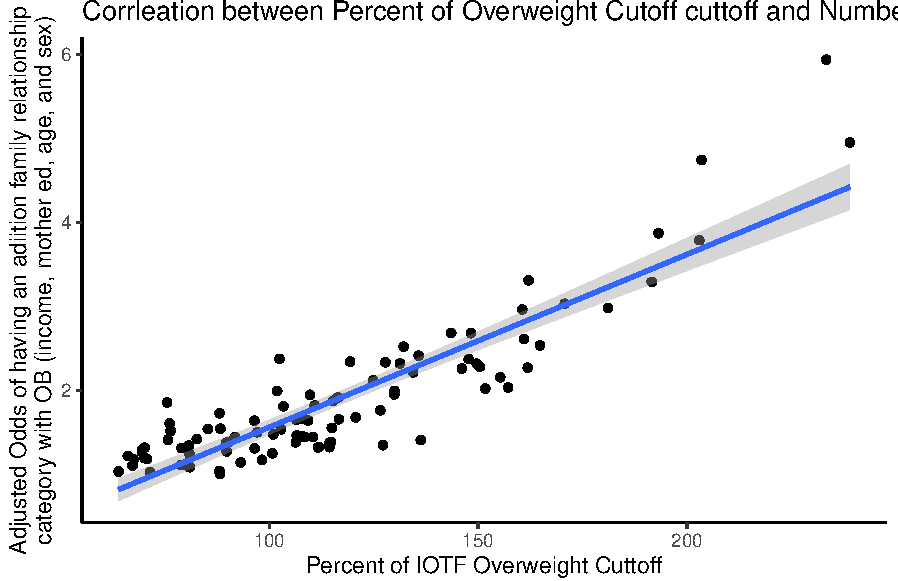
\includegraphics{UAE_MedPaper_Figs/fig-IOTF_pOWcutoff_nFamOB_adjOdds_plot-1.pdf}

\FloatBarrier
\clearpage

\hypertarget{sleep}{%
\section{Sleep}\label{sleep}}

\begin{table}[!h]

\caption{\label{tab:Beh_OB_tab}Sleep by Weight Status}
\centering
\begin{tabular}[t]{lllllll}
\toprule
Characteristic & N & HW & OW & OB & t-test & chi/fisher\\
\midrule
Bedtime\_cat & 97 &  &  &  &  & 0.274\\
\hspace{1em}7 - 8 pm &  & 11 (30\%) & 3 (12\%) & 6 (17\%) &  & \\
\hspace{1em}9 pm &  & 11 (30\%) & 7 (28\%) & 5 (14\%) &  & \\
\hspace{1em}10 pm &  & 9 (24\%) & 5 (20\%) & 10 (29\%) &  & \\
\hspace{1em}11 - Midnight &  & 3 (8.1\%) & 6 (24\%) & 9 (26\%) &  & \\
\addlinespace
\hspace{1em}After Midnight &  & 3 (8.1\%) & 4 (16\%) & 5 (14\%) &  & \\
\hspace{1em}Unknown &  & 4 & 4 & 2 &  & \\
Bed\_hr & 99 & 8.68 [2.00 - 11.50] & 8.48 [5.00 - 12.00] & 8.21 [6.00 - 11.00] & 0.482 & \\
\hspace{1em}Unknown &  & 2 & 4 & 2 &  & \\
CSHQ\_BedtimeResit & 94 & 7.77 [5.00 - 13.00] & 6.91 [5.00 - 11.00] & 7.19 [5.00 - 13.00] & 0.297 & \\
\addlinespace
\hspace{1em}Unknown &  & 6 & 6 & 1 &  & \\
CSHQ\_SleepOnsetDelay & 100 & 1.51 [1.00 - 3.00] & 1.62 [1.00 - 3.00] & 2.09 [1.00 - 3.00] & 0.009 & \\
\hspace{1em}Unknown &  & 2 & 3 & 2 &  & \\
CSHQ\_SleepDuration & 99 & 4.55 [3.00 - 8.00] & 4.52 [3.00 - 9.00] & 4.89 [3.00 - 9.00] & 0.620 & \\
\hspace{1em}Unknown &  & 3 & 4 & 1 &  & \\
\addlinespace
CSHQ\_SleepAnxiety & 98 & 6.13 [4.00 - 12.00] & 5.76 [4.00 - 12.00] & 5.14 [4.00 - 11.00] & 0.208 & \\
\hspace{1em}Unknown &  & 3 & 4 & 2 &  & \\
CSHQ\_NightWaking\_no16 & 96 & 2.89 [2.00 - 6.00] & 2.75 [2.00 - 6.00] & 3.09 [2.00 - 6.00] & 0.598 & \\
\hspace{1em}Unknown &  & 3 & 5 & 3 &  & \\
CSHQ\_Parasomnias & 93 & 8.67 [7.00 - 19.00] & 8.58 [7.00 - 12.00] & 9.21 [7.00 - 19.00] & 0.495 & \\
\addlinespace
\hspace{1em}Unknown &  & 5 & 5 & 4 &  & \\
CSHQ\_SleepDisorderBreathing & 95 & 2.53 [2.00 - 7.00] & 2.88 [2.00 - 6.00] & 3.41 [2.00 - 7.00] & 0.020 & \\
\hspace{1em}Unknown &  & 3 & 4 & 5 &  & \\
CSHQ\_DaytimeSleepiness & 91 & 13.14 [6.00 - 22.00] & 11.67 [7.00 - 18.00] & 12.52 [6.00 - 19.00] & 0.282 & \\
\hspace{1em}Unknown &  & 5 & 5 & 6 &  & \\
\bottomrule
\multicolumn{7}{l}{\rule{0pt}{1em}\textsuperscript{1} n (\%); Mean [Range]}\\
\end{tabular}
\end{table}

\FloatBarrier

\hypertarget{association-betwen-sleep-sub-scales-and-percent-of-overweight-cutoff}{%
\subsection{Association Betwen Sleep Sub-Scales and Percent of
Overweight
Cutoff}\label{association-betwen-sleep-sub-scales-and-percent-of-overweight-cutoff}}

\begin{table}[!h]

\caption{\label{tab:IOTF_pOWcutoff_sleep_cor}Correlations between sleep subscales and percent of overweight}
\centering
\begin{tabular}[t]{llllllllllll}
\toprule
  & IOTF\_pOWcutoff & Bedtime\_cMidnight & Bed\_hr & CSHQ\_BedtimeResit & CSHQ\_SleepOnsetDelay & CSHQ\_SleepDuration & CSHQ\_SleepAnxiety & CSHQ\_NightWaking\_no16 & CSHQ\_Parasomnias & CSHQ\_SleepDisorderBreathing & CSHQ\_DaytimeSleepiness\\
\midrule
IOTF\_pOWcutoff &  &  &  &  &  &  &  &  &  &  & \\
Bedtime\_cMidnight & 0.13 &  &  &  &  &  &  &  &  &  & \\
Bed\_hr & -0.09 & -0.48* &  &  &  &  &  &  &  &  & \\
CSHQ\_BedtimeResit & -0.13 & 0.1 & 0.01 &  &  &  &  &  &  &  & \\
CSHQ\_SleepOnsetDelay & 0.31* & 0.42* & -0.11 & 0.13 &  &  &  &  &  &  & \\
\addlinespace
CSHQ\_SleepDuration & 0.04 & 0.47* & -0.34* & 0.41* & 0.4* &  &  &  &  &  & \\
CSHQ\_SleepAnxiety & -0.18 & -0.16 & 0.24* & 0.62* & -0.1 & 0.02 &  &  &  &  & \\
CSHQ\_NightWaking\_no16 & 0.05 & -0.07 & 0.12 & 0.21 & 0.05 & 0.29* & 0.23* &  &  &  & \\
CSHQ\_Parasomnias & 0.04 & -0.06 & 0.06 & 0.17 & 0.02 & 0.04 & 0.12 & 0.41* &  &  & \\
CSHQ\_SleepDisorderBreathing & 0.32* & -0.03 & 0.02 & 0.25* & 0.04 & 0.07 & 0.19 & 0.36* & 0.45* &  & \\
\addlinespace
CSHQ\_DaytimeSleepiness & -0.04 & -0.07 & 0.09 & 0.28* & 0.16 & 0.21 & 0.28* & 0.05 & 0.18 & 0.13 & \\
\bottomrule
\end{tabular}
\end{table}
\FloatBarrier

Examining correlations between sleep sub-scales and percent of
overweight cutoff reveals greater percent of overweight cutoff was
associated with greater parent reported sleep onset delay and sleep
disordered breathing.

\FloatBarrier

\hypertarget{sensitivity-tests-1}{%
\subsubsection{Sensitivity Tests}\label{sensitivity-tests-1}}

\hypertarget{sleep-onset-delay}{%
\paragraph{Sleep Onset Delay}\label{sleep-onset-delay}}

\begin{table}[!h]

\caption{\label{tab:IOTF_pOWcutoff_sleepdelay}Linear Model: Sleep Onset Delay - SES category + Maternal Education + Age + Sex + pOWcutoff}
\centering
\begin{tabular}[t]{lrrrrl}
\toprule
  & b & se & t & p &  \\
\midrule
(Intercept) & 0.076 & 0.683 & 0.111 & 0.912 & \\
Month\_AED25,000 - 55,000 AED & -0.031 & 0.205 & -0.149 & 0.882 & \\
Month\_AED55,000 - 75,000 AED & -0.082 & 0.390 & -0.210 & 0.834 & \\
Month\_AED> 75,000 AED & -0.122 & 0.409 & -0.299 & 0.766 & \\
Mother\_ed & 0.008 & 0.029 & 0.261 & 0.795 & \\
\addlinespace
Age\_yr & 0.073 & 0.036 & 2.010 & 0.048 & *\\
sexM & 0.128 & 0.184 & 0.697 & 0.488 & \\
IOTF\_pOWcutoff & 0.006 & 0.003 & 2.126 & 0.037 & *\\
\bottomrule
\end{tabular}
\end{table}

After controlling for family income, mother education, child age, and
child sex, percent of overweight was positively associated with sleep
onset delay such that a child with 110\% of overweight, compared to
100\% of overweight, would be expected to have a sleep onset delay score
that was 0.06 points higher (range of scores = 0 - 3). Additionally, age
was positively associated with sleep onset delay such that each year
older, the expected sleep disordered breathing score would be 0.12
points higher (range of scores = 0 - 7).

\FloatBarrier

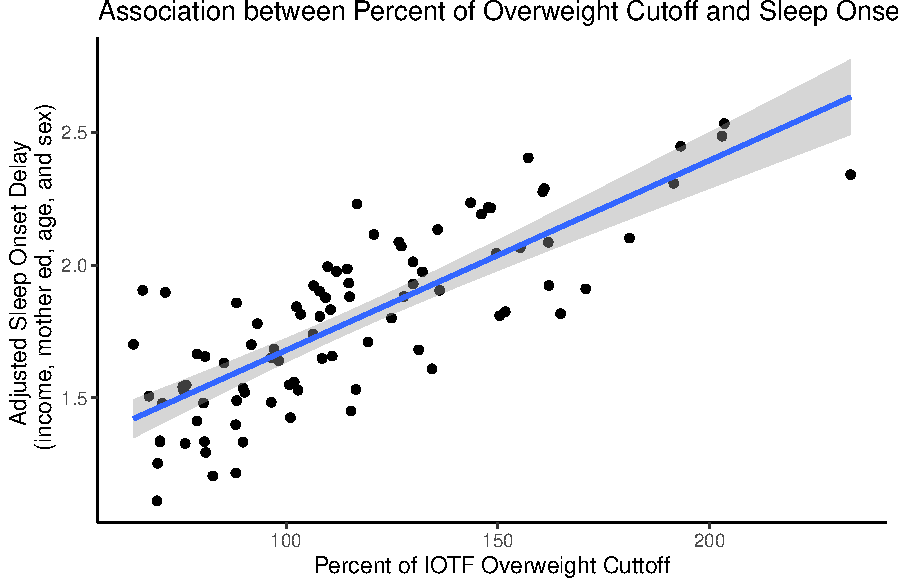
\includegraphics{UAE_MedPaper_Figs/fig-IOTF_pOWcutoff_sleepdelay_adj_plot-1.pdf}

\FloatBarrier

\FloatBarrier

\hypertarget{sleep-disordered-breathing}{%
\paragraph{Sleep Disordered
Breathing}\label{sleep-disordered-breathing}}

\begin{table}[!h]

\caption{\label{tab:IOTF_pOWcutoff_disbreathing}Linear Model: Sleep Disordered Breathing - SES category + Maternal Education + Age + Sex + pOWcutoff}
\centering
\begin{tabular}[t]{lrrrrl}
\toprule
  & b & se & t & p &  \\
\midrule
(Intercept) & 2.812 & 1.077 & 2.610 & 0.011 & \\
Month\_AED25,000 - 55,000 AED & -0.435 & 0.334 & -1.302 & 0.197 & \\
Month\_AED55,000 - 75,000 AED & -0.737 & 0.624 & -1.182 & 0.241 & \\
Month\_AED> 75,000 AED & -0.457 & 0.693 & -0.659 & 0.512 & \\
Mother\_ed & -0.012 & 0.047 & -0.259 & 0.796 & \\
\addlinespace
Age\_yr & -0.057 & 0.058 & -0.970 & 0.335 & \\
sexM & -0.001 & 0.298 & -0.004 & 0.996 & \\
IOTF\_pOWcutoff & 0.012 & 0.004 & 2.939 & 0.004 & **\\
\bottomrule
\end{tabular}
\end{table}

After controlling for family income, mother education, child age, and
child sex, percent of overweight was positively associated with sleep
disordered breathing such that a child with 110\% of overweight,
compared to 100\% of overweight, would be expected to have a sleep
disordered breathing score that was 0.12 points higher(range of scores =
2 - 7).

\FloatBarrier

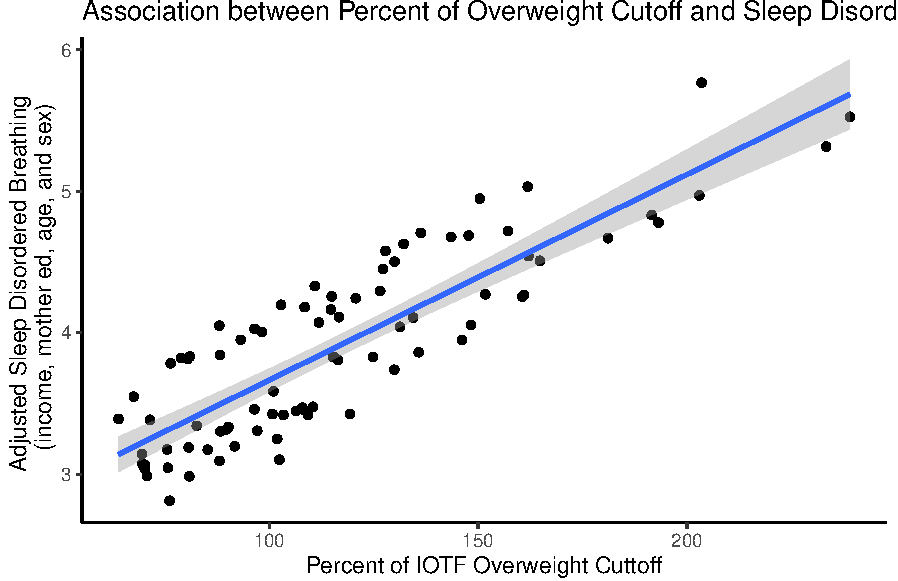
\includegraphics{UAE_MedPaper_Figs/fig-IOTF_pOWcutoff_disbreathing_adj_plot-1.pdf}

\FloatBarrier

\FloatBarrier

\clearpage

\hypertarget{strengths-and-difficulties-questionnaire}{%
\section{Strengths and Difficulties
Questionnaire}\label{strengths-and-difficulties-questionnaire}}

\begin{table}[!h]

\caption{\label{tab:SDQ_OB_tab}Strengths and Difficulties by Weight Status}
\centering
\begin{tabular}[t]{lllll}
\toprule
Characteristic & N & HW, N = 41 & OW, N = 29 & OB, N = 37\\
\midrule
SDQ\_EmotionProb\_raw & 104 & 3.05 [0.00 - 8.00] & 3.00 [0.00 - 7.00] & 3.43 [0.00 - 9.00]\\
\hspace{1em}Unknown &  & 2 & 1 & \vphantom{1} 0\\
SDQ\_ConductProb\_raw & 102 & 2.00 [0.00 - 7.00] & 1.68 [0.00 - 5.00] & 2.24 [0.00 - 6.00]\\
\hspace{1em}Unknown &  & 1 & 1 & \vphantom{1} 3\\
SDQ\_HyperactiveProb\_raw & 103 & 3.65 [0.00 - 9.00] & 3.07 [0.00 - 10.00] & 3.46 [0.00 - 10.00]\\
\addlinespace
\hspace{1em}Unknown &  & 2 & 2 & \vphantom{1} 0\\
SDQ\_PeerProb\_raw & 102 & 2.71 [0.00 - 7.00] & 2.97 [0.00 - 5.00] & 3.46 [1.00 - 6.00]\\
\hspace{1em}Unknown &  & 3 & 0 & \vphantom{1} 2\\
SDQ\_Prosocial\_raw & 102 & 8.47 [4.00 - 10.00] & 8.82 [6.00 - 10.00] & 8.11 [2.00 - 10.00]\\
\hspace{1em}Unknown &  & 2 & 1 & \vphantom{1} 2\\
\addlinespace
SDQ\_TotalProb\_raw & 106 & 11.11 [0.00 - 29.00] & 10.34 [4.00 - 20.00] & 12.22 [3.00 - 23.00]\\
\hspace{1em}Unknown &  & 1 & 0 & 0\\
SDQ\_TotalProb\_cat & 93 &  &  & \\
\hspace{1em}CloseToAverage &  & 27 (73\%) & 17 (68\%) & 19 (61\%)\\
\hspace{1em}High &  & 5 (14\%) & 2 (8.0\%) & 5 (16\%)\\
\addlinespace
\hspace{1em}SlightlyRaised &  & 3 (8.1\%) & 5 (20\%) & 4 (13\%)\\
\hspace{1em}VeryHigh &  & 2 (5.4\%) & 1 (4.0\%) & 3 (9.7\%)\\
\hspace{1em}Unknown &  & 4 & 4 & 6\\
SDQ\_EmotionProb\_cat & 104 &  &  & \\
\hspace{1em}CloseToAverage &  & 24 (62\%) & 18 (64\%) & 20 (54\%)\\
\addlinespace
\hspace{1em}High &  & 7 (18\%) & 5 (18\%) & 7 (19\%)\\
\hspace{1em}SlightlyRaised &  & 5 (13\%) & 3 (11\%) & 6 (16\%)\\
\hspace{1em}VeryHigh &  & 3 (7.7\%) & 2 (7.1\%) & 4 (11\%)\\
\hspace{1em}Unknown &  & 2 & 1 & 0\\
SDQ\_ConductProb\_cat & 102 &  &  & \\
\addlinespace
\hspace{1em}CloseToAverage &  & 26 (65\%) & 21 (75\%) & 22 (65\%)\\
\hspace{1em}High &  & 7 (18\%) & 4 (14\%) & 7 (21\%)\\
\hspace{1em}SlightlyRaised &  & 6 (15\%) & 3 (11\%) & 4 (12\%)\\
\hspace{1em}VeryHigh &  & 1 (2.5\%) & 0 (0\%) & 1 (2.9\%)\\
\hspace{1em}Unknown &  & 1 & 1 & 3\\
\addlinespace
SDQ\_HyperactivityProb\_cat & 103 &  &  & \\
\hspace{1em}CloseToAverage &  & 29 (74\%) & 24 (89\%) & 32 (86\%)\\
\hspace{1em}High &  & 1 (2.6\%) & 0 (0\%) & 0 (0\%)\\
\hspace{1em}SlightlyRaised &  & 8 (21\%) & 1 (3.7\%) & 3 (8.1\%)\\
\hspace{1em}VeryHigh &  & 1 (2.6\%) & 2 (7.4\%) & 2 (5.4\%)\\
\addlinespace
\hspace{1em}Unknown &  & 2 & 2 & 0\\
SDQ\_PeerProb\_cat & 102 &  &  & \\
\hspace{1em}CloseToAverage &  & 17 (45\%) & 12 (41\%) & 11 (31\%)\\
\hspace{1em}High &  & 10 (26\%) & 9 (31\%) & 11 (31\%)\\
\hspace{1em}SlightlyRaised &  & 7 (18\%) & 6 (21\%) & 7 (20\%)\\
\addlinespace
\hspace{1em}VeryHigh &  & 4 (11\%) & 2 (6.9\%) & 6 (17\%)\\
\hspace{1em}Unknown &  & 3 & 0 & 2\\
SDQ\_Prosocial\_cat & 102 &  &  & \\
\hspace{1em}CloseToAverage &  & 30 (77\%) & 22 (79\%) & 25 (71\%)\\
\hspace{1em}Low &  & 2 (5.1\%) & 2 (7.1\%) & 1 (2.9\%)\\
\addlinespace
\hspace{1em}SlightlyLowered &  & 5 (13\%) & 4 (14\%) & 6 (17\%)\\
\hspace{1em}VeryLow &  & 2 (5.1\%) & 0 (0\%) & 3 (8.6\%)\\
\hspace{1em}Unknown &  & 2 & 1 & 2\\
\bottomrule
\multicolumn{5}{l}{\rule{0pt}{1em}\textsuperscript{1} Mean [Range]; n (\%)}\\
\end{tabular}
\end{table}

There were no differences by weight status.

\hypertarget{exploratory-sex-x-percent-of-overweight-models}{%
\subsection{Exploratory Sex x Percent of Overweight
Models}\label{exploratory-sex-x-percent-of-overweight-models}}

\hypertarget{emotional-problems}{%
\subsubsection{Emotional Problems}\label{emotional-problems}}

Often complains of headaches

Many worries

Often unhappy, downhearted

Nervous or clingy in new situations

Many fears, easily scared

\FloatBarrier

\begin{table}[!h]

\caption{\label{tab:IOTF_pOWcutoff_emotprobs_elevated_logit}Logistic Model: Emotional Problems (Elevated vs Not) - SES category + Maternal Education + Age + Sex + pOWcutoff}
\centering
\begin{tabular}[t]{lrrrrrrrl}
\toprule
  & b & e\textasciicircum{}b & se & e\textasciicircum{}2.5 CI & e\textasciicircum{}97.5 CI & z & p &  \\
\midrule
(Intercept) & 0.554 & 1.740 & 1.740 & 0.057 & 5.520800e+01 & 0.318 & 0.750 & \\
Month\_AED25,000 - 55,000 AED & 0.013 & 1.013 & 0.531 & 0.359 & 2.932000e+00 & 0.024 & 0.981 & \\
Month\_AED55,000 - 75,000 AED & 0.369 & 1.446 & 1.049 & 0.155 & 1.134600e+01 & 0.351 & 0.725 & \\
Month\_AED> 75,000 AED & -16.635 & 0.000 & 1381.974 & NA & 3.271604e+40 & -0.012 & 0.990 & \\
Mother\_ed & -0.006 & 0.994 & 0.076 & 0.856 & 1.158000e+00 & -0.085 & 0.932 & .\\
\addlinespace
Age\_yr & -0.102 & 0.903 & 0.098 & 0.740 & 1.092000e+00 & -1.032 & 0.302 & \\
sexM & -0.096 & 0.909 & 0.537 & 0.309 & 2.599000e+00 & -0.178 & 0.858 & \\
IOTF\_pOWcutoff\_c100 & 0.011 & 1.011 & 0.010 & 0.992 & 1.032000e+00 & 1.155 & 0.248 & \\
sexM:IOTF\_pOWcutoff\_c100 & -0.005 & 0.995 & 0.013 & 0.969 & 1.020000e+00 & -0.420 & 0.675 & \\
\bottomrule
\end{tabular}
\end{table}

\FloatBarrier

\hypertarget{conduct-problems}{%
\subsection{Conduct Problems}\label{conduct-problems}}

Often has temper tantrums or hot tempers

Generally obedient - Reverse Scored

Often fights with other children

Often lies or cheats

Steals from home, school or elsewhere

\FloatBarrier

\begin{table}[!h]

\caption{\label{tab:IOTF_pOWcutoff_conductprobs_elevated_logit}Logistic Model: Conduct Problems (Elevated vs Not) - SES category + Maternal Education + Age + Sex + pOWcutoff}
\centering
\begin{tabular}[t]{lrrrrrrrl}
\toprule
  & b & e\textasciicircum{}b & se & e\textasciicircum{}2.5 CI & e\textasciicircum{}97.5 CI & z & p &  \\
\midrule
(Intercept) & -1.688 & 0.185 & 1.672 & 0.006 & 4.778 & -1.010 & 0.313 & \\
Month\_AED25,000 - 55,000 AED & -0.352 & 0.703 & 0.526 & 0.249 & 1.989 & -0.669 & 0.503 & \\
Month\_AED55,000 - 75,000 AED & 0.324 & 1.383 & 0.988 & 0.190 & 10.184 & 0.328 & 0.743 & \\
Month\_AED> 75,000 AED & -0.387 & 0.679 & 0.933 & 0.099 & 4.124 & -0.415 & 0.678 & \\
Mother\_ed & -0.005 & 0.995 & 0.074 & 0.857 & 1.152 & -0.069 & 0.945 & .\\
\addlinespace
Age\_yr & 0.137 & 1.147 & 0.095 & 0.954 & 1.389 & 1.443 & 0.149 & \\
sexM & -0.792 & 0.453 & 0.525 & 0.155 & 1.235 & -1.510 & 0.131 & \\
IOTF\_pOWcutoff\_c100 & -0.007 & 0.993 & 0.010 & 0.974 & 1.012 & -0.720 & 0.471 & \\
sexM:IOTF\_pOWcutoff\_c100 & 0.011 & 1.011 & 0.012 & 0.987 & 1.036 & 0.875 & 0.382 & \\
\bottomrule
\end{tabular}
\end{table}

\FloatBarrier

\hypertarget{hyperactivity}{%
\subsubsection{Hyperactivity}\label{hyperactivity}}

Restless, overactive

Constantly fidgeting or squirming

Easily distracted, concentration wanders

Thinks things out before acting - Reverse Scored

Sees tasks through to the end - Reverse Scored

\FloatBarrier

\begin{table}[!h]

\caption{\label{tab:IOTF_pOWcutoff_hypeprobs_elevated_logit}Logistic Model: Hyperactivity Problems (Elevated vs Not) - SES category + Maternal Education + Age + Sex + pOWcutoff}
\centering
\begin{tabular}[t]{lrrrrrrrl}
\toprule
  & b & e\textasciicircum{}b & se & e\textasciicircum{}2.5 CI & e\textasciicircum{}97.5 CI & z & p &  \\
\midrule
(Intercept) & 0.989 & 2.689 & 2.182 & 0.037 & 2.194150e+02 & 0.453 & 0.650 & \\
Month\_AED25,000 - 55,000 AED & -0.817 & 0.442 & 0.670 & 0.115 & 1.660000e+00 & -1.220 & 0.222 & \\
Month\_AED55,000 - 75,000 AED & -16.836 & 0.000 & 1584.870 & NA & 4.622569e+45 & -0.011 & 0.992 & \\
Month\_AED> 75,000 AED & 0.095 & 1.100 & 1.083 & 0.110 & 8.845000e+00 & 0.088 & 0.930 & \\
Mother\_ed & 0.011 & 1.011 & 0.096 & 0.840 & 1.233000e+00 & 0.110 & 0.912 & .\\
\addlinespace
Age\_yr & -0.155 & 0.856 & 0.126 & 0.659 & 1.089000e+00 & -1.234 & 0.217 & \\
sexM & -0.767 & 0.464 & 0.694 & 0.105 & 1.700000e+00 & -1.106 & 0.269 & \\
IOTF\_pOWcutoff\_c100 & -0.002 & 0.998 & 0.012 & 0.973 & 1.022000e+00 & -0.156 & 0.876 & \\
sexM:IOTF\_pOWcutoff\_c100 & 0.008 & 1.008 & 0.017 & 0.973 & 1.042000e+00 & 0.453 & 0.651 & \\
\bottomrule
\end{tabular}
\end{table}

\FloatBarrier

\hypertarget{peer-problems}{%
\subsubsection{Peer Problems}\label{peer-problems}}

Rather solitary, tends to play alone

Has at least one good friend - Reverse Scored

Generally liked by other children - Reverse Scored

Picked on or bullied

Gets on better with adults than with other children

\FloatBarrier

\begin{table}[!h]

\caption{\label{tab:IOTF_pOWcutoff_peerprobs_elevated_logit}Logistic Model: Peer Problems (Elevated vs Not) - SES category + Maternal Education + Age + Sex + pOWcutoff}
\centering
\begin{tabular}[t]{lrrrrrrrl}
\toprule
  & b & e\textasciicircum{}b & se & e\textasciicircum{}2.5 CI & e\textasciicircum{}97.5 CI & z & p &  \\
\midrule
(Intercept) & 0.048 & 1.049 & 1.806 & 0.030 & 38.161 & 0.026 & 0.979 & \\
Month\_AED25,000 - 55,000 AED & 0.212 & 1.236 & 0.546 & 0.421 & 3.650 & 0.388 & 0.698 & \\
Month\_AED55,000 - 75,000 AED & 2.186 & 8.896 & 1.294 & 0.931 & 215.972 & 1.689 & 0.091 & .\\
Month\_AED> 75,000 AED & 0.176 & 1.193 & 0.938 & 0.184 & 7.743 & 0.188 & 0.851 & \\
Mother\_ed & -0.151 & 0.860 & 0.087 & 0.716 & 1.011 & -1.726 & 0.084 & .\\
\addlinespace
Age\_yr & 0.152 & 1.164 & 0.101 & 0.959 & 1.431 & 1.497 & 0.134 & \\
sexM & 0.329 & 1.390 & 0.520 & 0.509 & 3.971 & 0.633 & 0.527 & *\\
IOTF\_pOWcutoff\_c100 & 0.024 & 1.024 & 0.012 & 1.002 & 1.050 & 2.047 & 0.041 & *\\
sexM:IOTF\_pOWcutoff\_c100 & -0.030 & 0.970 & 0.014 & 0.942 & 0.997 & -2.098 & 0.036 & *\\
\bottomrule
\end{tabular}
\end{table}

When examining odds of experiencing elevated peer problems, controlling
for family income, mother education, child age, and child sex, percent
of overweight, there was a significant sex x percent of overweight
interaction.

\FloatBarrier

\begin{verbatim}
sex = F:
 IOTF_pOWcutoff_c100 IOTF_pOWcutoff_c100.trend      SE  df asymp.LCL asymp.UCL
                  17                   0.02370 0.01158 Inf   0.00101    0.0464

sex = M:
 IOTF_pOWcutoff_c100 IOTF_pOWcutoff_c100.trend      SE  df asymp.LCL asymp.UCL
                  17                  -0.00632 0.00867 Inf  -0.02332    0.0107

Results are averaged over the levels of: Month_AED 
Confidence level used: 0.95 
\end{verbatim}

\FloatBarrier

For females, a female child with 110\% of overweight cutoff would have
1.27 times the odds of experiencing elevate peer problems than a female
child with 100\% of overweight cutoff. There was no association between
percent of overweight cutoff and odds of peer problems in males.

\FloatBarrier

\FloatBarrier

\hypertarget{prosocial}{%
\subsection{Prosocial}\label{prosocial}}

Considerate of other people's feelings

Shares readily with other children

Helpful if someone is hurt

Kind to younger children

Often volunteers to help others

\FloatBarrier

\begin{table}[!h]

\caption{\label{tab:IOTF_pOWcutoff_prosocialprobs_low_logit}Logistic Model: Prosocial Problems (Low vs Not) - SES category + Maternal Education + Age + Sex + pOWcutoff}
\centering
\begin{tabular}[t]{lrrrrrrrl}
\toprule
  & b & e\textasciicircum{}b & se & e\textasciicircum{}2.5 CI & e\textasciicircum{}97.5 CI & z & p &  \\
\midrule
(Intercept) & -1.501 & 0.223 & 2.020 & 0.004 & 11.541 & -0.743 & 0.457 & \\
Month\_AED25,000 - 55,000 AED & 0.018 & 1.018 & 0.647 & 0.292 & 3.825 & 0.027 & 0.978 & \\
Month\_AED55,000 - 75,000 AED & -0.611 & 0.543 & 1.413 & 0.018 & 6.626 & -0.433 & 0.665 & \\
Month\_AED> 75,000 AED & 1.766 & 5.849 & 1.048 & 0.772 & 50.723 & 1.686 & 0.092 & .\\
Mother\_ed & -0.037 & 0.964 & 0.085 & 0.810 & 1.139 & -0.435 & 0.664 & \\
\addlinespace
Age\_yr & 0.072 & 1.075 & 0.117 & 0.855 & 1.359 & 0.615 & 0.538 & \\
sexM & -1.479 & 0.228 & 0.772 & 0.041 & 0.908 & -1.916 & 0.055 & *\\
IOTF\_pOWcutoff\_c100 & -0.004 & 0.996 & 0.011 & 0.973 & 1.017 & -0.384 & 0.701 & \\
sexM:IOTF\_pOWcutoff\_c100 & 0.029 & 1.029 & 0.015 & 1.001 & 1.063 & 1.914 & 0.056 & .\\
\bottomrule
\end{tabular}
\end{table}

\clearpage
\FloatBarrier

\hypertarget{extra-tables-by-sex}{%
\section{Extra Tables by Sex}\label{extra-tables-by-sex}}

\FloatBarrier

\hypertarget{participant-characteristics-1}{%
\subsection{Participant
Characteristics}\label{participant-characteristics-1}}

\begin{table}[!h]

\caption{\label{tab:Demo_sex_tab}Demographic Characteristics by Sex}
\centering
\begin{tabular}[t]{llllll}
\toprule
Characteristic & N & F & M & t-test & chi/fisher\\
\midrule
Age\_yr & 107 & 12.79 (2.84)   [7.31 - 17.84] & 12.70 (2.57)   [8.04 - 17.54] & 0.875 & \\
BMI & 107 & 24.85 (7.94)   [12.71 - 47.60] & 25.70 (10.34)   [13.60 - 55.52] & 0.646 & \\
IOTF\_pOWcutoff & 107 & 112.22 (31.68)   [67.29 - 193.18] & 117.71 (43.37)   [63.95 - 239.00] & 0.471 & \\
IOTF\_WeightStatus & 107 &  &  &  & 0.454\\
\hspace{1em}Thinness2 &  & 1 (1.6\%) & 2 (4.3\%) &  & \\
\addlinespace
\hspace{1em}Thinness1 &  & 5 (8.2\%) & 3 (6.5\%) &  & \\
\hspace{1em}HW &  & 18 (30\%) & 12 (26\%) &  & \\
\hspace{1em}Overweight &  & 14 (23\%) & 15 (33\%) &  & \\
\hspace{1em}Obese &  & 11 (18\%) & 3 (6.5\%) &  & \\
\hspace{1em}MorbidlyObese &  & 12 (20\%) & 11 (24\%) &  & \\
\addlinespace
Father\_ed & 102 & 13.08 (3.79)   [0.00 - 18.00] & 12.48 (3.14)   [6.00 - 18.00] & 0.384 & \\
\hspace{1em}Unknown &  & 3 & 2 &  & \\
Mother\_ed & 99 & 13.14 (3.56)   [3.00 - 18.00] & 13.24 (3.04)   [0.00 - 18.00] & 0.884 & \\
\hspace{1em}Unknown &  & 4 & 4 &  & \\
Month\_AED & 99 &  &  &  & 0.745\\
\addlinespace
\hspace{1em}<25,000 AED &  & 15 (27\%) & 16 (37\%) &  & \\
\hspace{1em}25,000 - 55,000 AED &  & 32 (57\%) & 21 (49\%) &  & \\
\hspace{1em}55,000 - 75,000 AED &  & 4 (7.1\%) & 2 (4.7\%) &  & \\
\hspace{1em}> 75,000 AED &  & 5 (8.9\%) & 4 (9.3\%) &  & \\
\hspace{1em}Unknown &  & 5 & 3 &  & \\
\addlinespace
DadNationality & 101 &  &  &  & 1.00\\
\hspace{1em}Emirati &  & 58 (97\%) & 40 (98\%) &  & \\
\hspace{1em}Omani &  & 1 (1.7\%) & 0 (0\%) &  \vphantom{1} & \\
\hspace{1em}Yemeni &  & 1 (1.7\%) & 1 (2.4\%) &  & \\
\hspace{1em}Unknown &  & 1 & 5 &  & \\
\addlinespace
MomNationality & 104 &  &  &  & 0.526\\
\hspace{1em}Emirati &  & 55 (92\%) & 41 (93\%) &  & \\
\hspace{1em}Omani &  & 1 (1.7\%) & 0 (0\%) &  & \\
\hspace{1em}Yemeni &  & 0 (0\%) & 1 (2.3\%) &  & \\
\hspace{1em}Moroccan &  & 2 (3.3\%) & 0 (0\%) &  & \\
\addlinespace
\hspace{1em}Egyptian &  & 2 (3.3\%) & 1 (2.3\%) &  & \\
\hspace{1em}Bahrani &  & 0 (0\%) & 1 (2.3\%) &  & \\
\hspace{1em}Unknown &  & 1 & 2 &  & \\
\bottomrule
\multicolumn{6}{l}{\rule{0pt}{1em}\textsuperscript{1} Mean (SD)   [Range]; n (\%)}\\
\end{tabular}
\end{table}

There were no differences by sex with the exception of females having a
higher hip-to-waist ratio, which would be expected for this age range.

\FloatBarrier
\clearpage

\hypertarget{medical-comorbidities-1}{%
\subsection{Medical Comorbidities}\label{medical-comorbidities-1}}

\begin{table}[!h]

\caption{\label{tab:Med_sex_tab}Medical Comorbidities by Weight Status}
\centering
\begin{tabular}[t]{llllll}
\toprule
Characteristic & N & F & M & t-test & chi/fisher\\
\midrule
nComorbid & 107 & 2.25 (1.07)   [0.00 - 4.00] & 2.02 (0.98)   [0.00 - 4.00] & 0.263 & \\
VitDdeficiency & 107 &  &  &  & 1.00\\
\hspace{1em}Y &  & 56 (92\%) & 42 (91\%) &  & \\
\hspace{1em}N &  & 5 (8.2\%) & 4 (8.7\%) &  & \\
Anemia & 40 &  &  &  & 0.424\\
\addlinespace
\hspace{1em}Iron Deficiency Anemia (ID) &  & 13 (54\%) & 8 (50\%) &  & \\
\hspace{1em}Thalassemia Minor (TM) &  & 2 (8.3\%) & 1 (6.2\%) &  & \\
\hspace{1em}G6PD Deficiency &  & 0 (0\%) & 1 (6.2\%) &  & \\
\hspace{1em}ID + TM &  & 0 (0\%) & 2 (12\%) &  & \\
\hspace{1em}ID + G6PD Deficiency &  & 1 (4.2\%) & 0 (0\%) &  & \\
\addlinespace
\hspace{1em}Unspecified Anemia &  & 8 (33\%) & 4 (25\%) &  & \\
\hspace{1em}Unknown &  & 37 & 30 &  & \\
Hyperlipidemia & 12 &  &  &  & 1.00\\
\hspace{1em}Hyperlipidemia &  & 8 (89\%) & 3 (100\%) &  & \\
\hspace{1em}Hyperlipidemia - Mixed &  & 1 (11\%) & 0 (0\%) &  & \\
\addlinespace
\hspace{1em}Unknown &  & 52 & 43 &  & \\
ThyroidConditions & 25 &  &  &  & 1.00\\
\hspace{1em}Abnormal Function &  & 10 (56\%) & 4 (57\%) &  & \\
\hspace{1em}Autoimmune Thyroiditis &  & 3 (17\%) & 2 (29\%) &  & \\
\hspace{1em}Autoimmune Hypothyroidism &  & 0 (0\%) & 0 (0\%) &  & \\
\addlinespace
\hspace{1em}Unspecified Hypothyroidism &  & 4 (22\%) & 1 (14\%) &  & \\
\hspace{1em}Goiter &  & 1 (5.6\%) & 0 (0\%) &  & \\
\hspace{1em}Unknown &  & 43 & 39 &  & \\
GlycemicStatus & 28 &  &  &  & 0.678\\
\hspace{1em}Impaired Fasting Glucose &  & 9 (64\%) & 10 (71\%) &  & \\
\addlinespace
\hspace{1em}Impaired Glucose Tolerance Test &  & 3 (21\%) & 4 (29\%) &  & \\
\hspace{1em}Type-1 Diabetes &  & 2 (14\%) & 0 (0\%) &  & \\
\hspace{1em}Unknown &  & 47 & 32 &  & \\
Acanthosis Nigricans & 8 & 6 (100\%) & 2 (100\%) &  & \\
\hspace{1em}Unknown &  & 55 & 44 &  & \\
\addlinespace
Hypertension & 3 &  &  &  & \\
\hspace{1em}Essential Primary Hypertension &  & 1 (100\%) & 1 (50\%) &  & \\
\hspace{1em}High Blood Pressure &  & 0 (0\%) & 1 (50\%) &  & \\
\hspace{1em}Unknown &  & 60 & 44 &  & \\
Metabolic Syndrome & 2 & 1 (100\%) & 1 (100\%) &  & \\
\addlinespace
\hspace{1em}Unknown &  & 60 & 45 &  & \\
Growth.Stature & 10 &  &  &  & 1.00\\
\hspace{1em}Failure To Thrive (FT) &  & 0 (0\%) & 1 (17\%) &  & \\
\hspace{1em}Growth Hormone Deficency &  & 0 (0\%) & 1 (17\%) &  & \\
\hspace{1em}Short Stature &  & 3 (75\%) & 3 (50\%) &  & \\
\addlinespace
\hspace{1em}FT + ShortStature + Underweight &  & 1 (25\%) & 0 (0\%) &  & \\
\hspace{1em}Short Stature + Precocious Puberty &  & 0 (0\%) & 1 (17\%) &  & \\
\hspace{1em}Unknown &  & 57 & 40 &  & \\
PCOS & 4 &  &  &  & \\
\hspace{1em}PCOS &  & 2 (50\%) & 0 (NA\%) &  & \\
\addlinespace
\hspace{1em}Hirsutism &  & 1 (25\%) & 0 (NA\%) &  & \\
\hspace{1em}Hirsutism + Unspecified Ovarian Cysts &  & 1 (25\%) & 0 (NA\%) &  & \\
\hspace{1em}Unknown &  & 57 & 46 &  & \\
\bottomrule
\multicolumn{6}{l}{\rule{0pt}{1em}\textsuperscript{1} Mean (SD)   [Range]; n (\%)}\\
\end{tabular}
\end{table}

Presence of different co-morbidities did not differ by sex, nor did the
number of co-morbidities

\FloatBarrier
\clearpage

\hypertarget{family-history-1}{%
\subsection{Family History}\label{family-history-1}}

\begin{table}[!h]

\caption{\label{tab:Fam_sex_tab}Family History by Sex}
\centering
\begin{tabular}[t]{llllll}
\toprule
Characteristic & N & F & M & t-test & chi/fisher\\
\midrule
Fam\_OB\_YN & 101 &  &  &  & 0.895\\
\hspace{1em}yes &  & 41 (71\%) & 29 (67\%) &  & \\
\hspace{1em}no &  & 17 (29\%) & 14 (33\%) &  & \\
\hspace{1em}Unknown &  & 3 & 3 &  & \\
nFam\_Obesity & 107 & 1.80 (1.80)   [0.00 - 7.00] & 1.80 (1.71)   [0.00 - 5.00] & 1.00 & \\
\addlinespace
Mother & 107 & 11 (18\%) & 7 (15\%) &  & \\
Father & 107 & 9 (15\%) & 12 (26\%) &  & \\
Grandmother & 107 & 19 (31\%) & 14 (30\%) &  & \\
Grandfather & 107 & 4 (6.6\%) & 2 (4.3\%) &  & \\
Sister & 107 & 10 (16\%) & 6 (13\%) &  & \\
\addlinespace
Brother & 107 & 15 (25\%) & 10 (22\%) &  & \\
Aunt & 107 & 26 (43\%) & 19 (41\%) &  & \\
Uncle & 107 & 16 (26\%) & 13 (28\%) &  & \\
Fam\_ED\_YN & 96 &  &  &  & 0.517\\
\hspace{1em}yes &  & 5 (8.9\%) & 6 (15\%) &  & \\
\addlinespace
\hspace{1em}no &  & 51 (91\%) & 34 (85\%) &  & \\
\hspace{1em}Unknown &  & 5 & 6 &  & \\
nFam\_EatingDisorder & 107 & 0.21 (0.97)   [0.00 - 7.00] & 0.22 (0.63)   [0.00 - 3.00] & 0.98 & \\
Mother & 107 & 1 (1.6\%) & 0 (0\%) &  & \\
Father & 107 & 1 (1.6\%) & 1 (2.2\%) &  & \\
\addlinespace
Grandmother & 107 & 2 (3.3\%) & 2 (4.3\%) &  & \\
Grandfather & 107 & 2 (3.3\%) & 0 (0\%) &  & \\
Sister & 107 & 2 (3.3\%) & 0 (0\%) &  & \\
Brother & 107 & 1 (1.6\%) & 1 (2.2\%) &  & \\
Aunt & 107 & 3 (4.9\%) & 4 (8.7\%) &  & \\
\addlinespace
Uncle & 107 & 1 (1.6\%) & 2 (4.3\%) &  & \\
\bottomrule
\multicolumn{6}{l}{\rule{0pt}{1em}\textsuperscript{1} n (\%); Mean (SD)   [Range]}\\
\end{tabular}
\end{table}

There were no differences by sex.

\FloatBarrier
\clearpage

\hypertarget{sleep-1}{%
\subsection{Sleep}\label{sleep-1}}

\begin{table}[!h]

\caption{\label{tab:Beh_sex_tab}Sleep by Sex}
\centering
\begin{tabular}[t]{llllll}
\toprule
Characteristic & N & F & M & t-test & chi/fisher\\
\midrule
Bedtime\_cat & 97 &  &  &  & 0.151\\
\hspace{1em}7 - 8 pm &  & 12 (21\%) & 8 (20\%) &  & \\
\hspace{1em}9 pm &  & 9 (16\%) & 14 (34\%) &  & \\
\hspace{1em}10 pm &  & 15 (27\%) & 9 (22\%) &  & \\
\hspace{1em}11 - Midnight &  & 14 (25\%) & 4 (9.8\%) &  & \\
\addlinespace
\hspace{1em}After Midnight &  & 6 (11\%) & 6 (15\%) &  & \\
\hspace{1em}Unknown &  & 5 & 5 &  & \\
Bed\_hr & 99 & 8.55 (1.54)   [6.00 - 12.00] & 8.35 (1.80)   [2.00 - 11.50] & 0.548 & \\
\hspace{1em}Unknown &  & 4 & 4 &  \vphantom{1} & \\
CSHQ\_BedtimeResit & 94 & 7.72 (2.10)   [5.00 - 13.00] & 6.85 (2.17)   [5.00 - 13.00] & 0.056 & \\
\addlinespace
\hspace{1em}Unknown &  & 8 & 5 &  & \\
CSHQ\_SleepOnsetDelay & 100 & 1.69 (0.86)   [1.00 - 3.00] & 1.81 (0.83)   [1.00 - 3.00] & 0.486 & \\
\hspace{1em}Unknown &  & 3 & 4 &  & \\
CSHQ\_SleepDuration & 99 & 4.86 (1.62)   [3.00 - 9.00] & 4.40 (1.80)   [3.00 - 9.00] & 0.198 & \\
\hspace{1em}Unknown &  & 4 & 4 &  & \\
\addlinespace
CSHQ\_SleepAnxiety & 98 & 6.02 (2.58)   [4.00 - 12.00] & 5.24 (2.05)   [4.00 - 11.00] & 0.099 & \\
\hspace{1em}Unknown &  & 5 & 4 &  & \\
CSHQ\_NightWaking\_no16 & 96 & 3.11 (1.36)   [2.00 - 6.00] & 2.68 (1.11)   [2.00 - 6.00] & 0.094 & \\
\hspace{1em}Unknown &  & 6 & 5 &  & \\
CSHQ\_Parasomnias & 93 & 8.75 (2.26)   [7.00 - 19.00] & 8.97 (2.26)   [7.00 - 19.00] & 0.634 & \\
\addlinespace
\hspace{1em}Unknown &  & 6 & 8 &  & \\
CSHQ\_SleepDisorderBreathing & 95 & 2.87 (1.24)   [2.00 - 7.00] & 2.98 (1.44)   [2.00 - 7.00] & 0.710 & \\
\hspace{1em}Unknown &  & 7 & 5 &  & \\
CSHQ\_DaytimeSleepiness & 91 & 12.64 (3.35)   [6.00 - 18.00] & 12.39 (3.74)   [6.00 - 22.00] & 0.747 & \\
\hspace{1em}Unknown &  & 8 & 8 &  & \\
\addlinespace
CSHQ\_Total\_no16 & 72 & 46.51 (7.52)   [34.00 - 63.00] & 44.73 (8.74)   [32.00 - 71.00] & 0.361 & \\
\hspace{1em}Unknown &  & 22 & 13 &  & \\
\bottomrule
\multicolumn{6}{l}{\rule{0pt}{1em}\textsuperscript{1} n (\%); Mean (SD)   [Range]}\\
\end{tabular}
\end{table}

There were no differences by sex.

\FloatBarrier
\clearpage

\hypertarget{strengths-and-difficulties-questionnaire-1}{%
\subsection{Strengths and Difficulties
Questionnaire}\label{strengths-and-difficulties-questionnaire-1}}

\begin{table}[!h]

\caption{\label{tab:SDQ_sex_tab}Strengths and Difficulty by Sex}
\centering
\begin{tabular}[t]{llllll}
\toprule
Characteristic & N & F & M & t-test & chi/fisher\\
\midrule
SDQ\_EmotionProb\_raw & 104 & 3.54 (2.17)   [0.00 - 9.00] & 2.69 (2.22)   [0.00 - 8.00] & 0.053 & \\
\hspace{1em}Unknown &  & 2 & 1 &  \vphantom{1} & \\
SDQ\_ConductProb\_raw & 102 & 2.00 (1.66)   [0.00 - 6.00] & 1.98 (1.71)   [0.00 - 7.00] & 0.945 & \\
\hspace{1em}Unknown &  & 2 & 3 &  \vphantom{3} & \\
SDQ\_HyperactiveProb\_raw & 103 & 3.12 (2.31)   [0.00 - 10.00] & 3.85 (2.37)   [0.00 - 10.00] & 0.120 & \\
\addlinespace
\hspace{1em}Unknown &  & 2 & 2 &  \vphantom{1} & \\
SDQ\_PeerProb\_raw & 102 & 2.85 (1.42)   [0.00 - 5.00] & 3.30 (1.49)   [0.00 - 7.00] & 0.124 & \\
\hspace{1em}Unknown &  & 2 & 3 &  \vphantom{2} & \\
SDQ\_Prosocial\_raw & 102 & 8.38 (1.46)   [4.00 - 10.00] & 8.53 (1.93)   [2.00 - 10.00] & 0.659 & \\
\hspace{1em}Unknown &  & 3 & 2 &  \vphantom{1} & \\
\addlinespace
SDQ\_TotalProb\_raw & 106 & 11.13 (5.05)   [0.00 - 23.00] & 11.50 (5.65)   [3.00 - 29.00] & 0.729 & \\
\hspace{1em}Unknown &  & 0 & 1 &  & \\
SDQ\_TotalProb\_cat & 93 &  &  &  & 0.411\\
\hspace{1em}CloseToAverage &  & 37 (71\%) & 26 (63\%) &  & \\
\hspace{1em}High &  & 8 (15\%) & 4 (9.8\%) &  & \\
\addlinespace
\hspace{1em}SlightlyRaised &  & 5 (9.6\%) & 7 (17\%) &  & \\
\hspace{1em}VeryHigh &  & 2 (3.8\%) & 4 (9.8\%) &  & \\
\hspace{1em}Unknown &  & 9 & 5 &  & \\
SDQ\_EmotionProb\_cat & 104 &  &  &  & 0.347\\
\hspace{1em}CloseToAverage &  & 31 (53\%) & 31 (69\%) &  & \\
\addlinespace
\hspace{1em}High &  & 13 (22\%) & 6 (13\%) &  & \\
\hspace{1em}SlightlyRaised &  & 10 (17\%) & 4 (8.9\%) &  & \\
\hspace{1em}VeryHigh &  & 5 (8.5\%) & 4 (8.9\%) &  & \\
\hspace{1em}Unknown &  & 2 & 1 &  & \\
SDQ\_ConductProb\_cat & 102 &  &  &  & 0.98\\
\addlinespace
\hspace{1em}CloseToAverage &  & 40 (68\%) & 29 (67\%) &  & \\
\hspace{1em}High &  & 11 (19\%) & 7 (16\%) &  & \\
\hspace{1em}SlightlyRaised &  & 7 (12\%) & 6 (14\%) &  & \\
\hspace{1em}VeryHigh &  & 1 (1.7\%) & 1 (2.3\%) &  & \\
\hspace{1em}Unknown &  & 2 & 3 &  \vphantom{1} & \\
\addlinespace
SDQ\_HyperactivityProb\_cat & 103 &  &  &  & 0.704\\
\hspace{1em}CloseToAverage &  & 48 (81\%) & 37 (84\%) &  & \\
\hspace{1em}High &  & 0 (0\%) & 1 (2.3\%) &  & \\
\hspace{1em}SlightlyRaised &  & 8 (14\%) & 4 (9.1\%) &  & \\
\hspace{1em}VeryHigh &  & 3 (5.1\%) & 2 (4.5\%) &  & \\
\addlinespace
\hspace{1em}Unknown &  & 2 & 2 &  & \\
SDQ\_PeerProb\_cat & 102 &  &  &  & 0.312\\
\hspace{1em}CloseToAverage &  & 23 (39\%) & 17 (40\%) &  & \\
\hspace{1em}High &  & 19 (32\%) & 11 (26\%) &  & \\
\hspace{1em}SlightlyRaised &  & 13 (22\%) & 7 (16\%) &  & \\
\addlinespace
\hspace{1em}VeryHigh &  & 4 (6.8\%) & 8 (19\%) &  & \\
\hspace{1em}Unknown &  & 2 & 3 &  & \\
SDQ\_Prosocial\_cat & 102 &  &  &  & 0.482\\
\hspace{1em}CloseToAverage &  & 42 (72\%) & 35 (80\%) &  & \\
\hspace{1em}Low &  & 3 (5.2\%) & 2 (4.5\%) &  & \\
\addlinespace
\hspace{1em}SlightlyLowered &  & 11 (19\%) & 4 (9.1\%) &  & \\
\hspace{1em}VeryLow &  & 2 (3.4\%) & 3 (6.8\%) &  & \\
\hspace{1em}Unknown &  & 3 & 2 &  & \\
\bottomrule
\multicolumn{6}{l}{\rule{0pt}{1em}\textsuperscript{1} Mean (SD)   [Range]; n (\%)}\\
\end{tabular}
\end{table}

There were no differences by sex.

\FloatBarrier
\clearpage

\textbackslash end\{document\}

\end{document}
